In the following sections, we present and discuss both the determination of optimal parameters for the localization model and the construction of the coloration models based on the data collected in the listening experiments described above.

%% Localization results
\subsection{Comparison of localization models}\label{sec:05_Proposed_Models:Localization_Results}
Using the measured perceived source directions from the localization experiment (described in \secref{sec:05_Proposed_Models:Localization_Test}), we first determined optimal parameter values (for each of the 4 parameters discussed in \secref{sec:05_Proposed_Models:Localization_Model}) separately for both the velocity and energy vector models.
The optimization consisted of minimizing the squared-residuals between the predicted and measured localization azimuths.
The resulting parameter values are listed in \tabref{tab:Vector_Parameters}.
From these optimal values, we see that, generally, the low-frequency (velocity) vector requires a ``coarser'' set of input data, as the spatial resolution (related to $Q$) is much lower.
Conceptually, this agrees with the notion that low-frequency sounds are not very directional, so a low-spatial-resolution representation of such information should be adequate.
Similarly, the wavelet lengths (set by $\tau_\text{w}$) are longer for the velocity vector than for the energy vector, which is likely a result of low-frequency information requiring longer time-scales in order to be adequately represented.

\begin{table}[t]
\centering
 \begin{tabular}{|c|c|c|c|} \hline
 \textbf{Parameter} & \textbf{Velocity} & \textbf{Energy} & \textbf{Description} \\ \hline
 $Q$ & 9 & 36 & Number of plane-waves \\
 $\alpha$ & 0.95 & 0.7 & Stationary signal weight \\
 $\tau_\text{w}$~(ms) & 2 & 1 & Minimum wavelet half-length \\
 $G_\text{min}$~(dB) & $-8$ & $-30$ & Wavelet detection threshold \\ \hline
 \end{tabular}
 \caption[Optimal parameters for the proposed localization model.]{
 Optimal parameters for each localization vector (velocity and energy).
 More detailed descriptions of each parameter are given in \secref{sec:05_Proposed_Models:Localization_Model}.}
 \label{tab:Vector_Parameters}
\end{table}

In \figref{fig:Localization_Model_Comparison}, the measured localization directions are plotted against the predictions of each model.
The mean absolute prediction error is given by
\begin{equation}
\bar{\epsilon} = \frac{1}{N_\text{r}} \sum_{j = 1}^{N_\text{r}} | \phi_j - \phi_p |,
\end{equation}
where $N_\text{r}$ is the total number of responses, $\phi_j$ is the measured azimuth for response $j$, and $\phi_p$ is the predicted azimuth.
These errors, as well as the squared residuals and Pearson correlation coefficients for the data, are given in \tabref{tab:Localization_Model_Results}.
From these values, we see that the proposed model seems to better predict the data than does the binaural model, as the former achieves a lower squared-residual value, a higher correlation with the data, and a smaller mean absolute prediction error.
This is somewhat surprising given the binaural model's capacity to take into account both subject-dependent variations, since the predictions are made on a per-subject basis (see \secref{sec:04_Auditory_Models:Binaural_Localization_Model}), as well as any effects of the binaural rendering approach used.
The proposed model, on the other hand, is unaware of the binaural rendering approach used and can only make a single prediction per sample, meaning that any subject-dependent variation in the data cannot be captured.
However, unlike the proposed model, the binaural model does not have any free parameters and, accordingly, did not need to be tuned to fit the data.

\begin{table}[t]
\centering
 \begin{tabular}{|c|c|c|c|} \hline
 \textbf{Model Name} & \textbf{Residuals} & \textbf{Correlation} & $\bar{\epsilon}$ \\ \hline
 Proposed & 706.5 & 0.85 & $3.67^\circ$ \\
 \citet{Dietz2011} & 877.0 & 0.81 & $4.36^\circ$ \\ \hline
 \end{tabular}
 \caption[Prediction errors and correlation coefficients for each localization model.]{
 Squared residuals, Pearson correlation coefficients, and mean absolute prediction errors ($\bar{\epsilon}$) for each localization model.
 The squared residuals are normalized by the variance seen in the measured data for each sample.}
 \label{tab:Localization_Model_Results}
\end{table}

\begin{figure}[t]
\centering
  \begin{subfigure}[b]{0.49\columnwidth}
        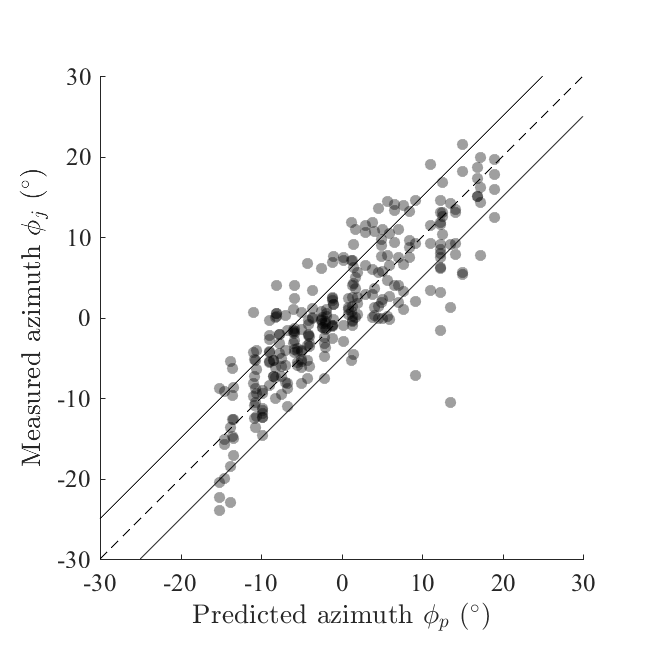
\includegraphics[width=\textwidth]{05_proposed_models/figures/LocalizationModelResults}
        \caption{Proposed model}
        \label{fig:Localization_Model_Results}
  \end{subfigure}
  \hfill
  \begin{subfigure}[b]{0.49\columnwidth}
        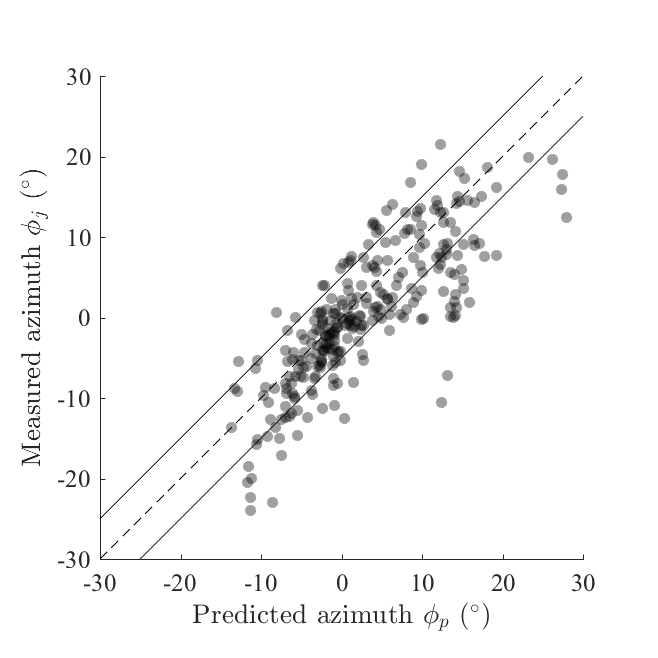
\includegraphics[width=\textwidth]{05_proposed_models/figures/DietzLocalizationResults}
        \caption{\citet{Dietz2011} model}
        \label{fig:Dietz_Localization_Results}
  \end{subfigure}
  \caption[Scatter plots of measured versus predicted source directions.]{
  Scatter plots of measured versus predicted source directions.
  The transparent filled circles indicate the data and model values;
  the dashed lines indicate ideal model results (i.e., $\phi_j = \phi_p$);
  the solid lines indicate discrepancies of $5^\circ$ (i.e., $\phi_j = \phi_p \pm 5^\circ$).}
  \label{fig:Localization_Model_Comparison}
\end{figure}

For both models we observe two outlying data points at approximately $(\phi_p, \phi_j) = (+10^\circ, -10^\circ)$, for which the predicted directions are to the listener's left ($+$), while that subject (both of these data points are from the same subject) localized the sound to the right ($-$).
Although not shown here, the same data points appear again as outliers when plotted against the \textit{intended} source direction, suggesting that these outliers could well be due to an error on the part of the subject.

%% Coloration results
\subsection{Comparison of coloration models}\label{sec:05_Proposed_Models:Coloration_Results}
Using the MUSHRA ratings collected from the coloration listening test (described in \secref{sec:05_Proposed_Models:Coloration_Test}), we performed linear regressions for each model listed in \secref{sec:05_Proposed_Models:Coloration_Models}.
We first converted the MUSHRA ratings to ``coloration scores'', given by $C = 100 - M$, where $M$ are the MUSHRA ratings.
Through this transformation, a reference sample will always have a coloration score of zero, while the low-pass anchor will have a coloration score of 100.
We then computed linear regressions between the values of the metrics in each of the four models and the coloration scores.
Note that, for the binaural models (\citet{Pulkki1999} and \citet{Wittek2007}), we computed each metric on a per-subject basis, i.e., using each subject's individualized HRTFs to render to binaural and subsequently computing per-subject values of each metric.

In building the coloration models, an analysis of the statistical significance of each model parameter revealed that, for the proposed model, neither $\sigma_\eta$ nor $E_{\text{pk}}$ provided a significant improvement to the model.
This is likely because, for all of our test samples, both $\sigma_\eta$ and $E_{\text{pk}}$ were strongly correlated with $\rho_\eta$.
Consequently, our proposed model uses only $\rho_\eta$ and $E_\text{n}$.
Additionally, a ``$y$-intercept'' (offset) term was considered for each model, but was found to be statistically insignificant in all cases.%
\footnote{This is likely because all of the reference samples, by definition, obtain zero coloration scores and zero values for each metric.}
The final formulae and corresponding Pearson correlation coefficients between the measured and predicted coloration scores are tabulated in \tabref{tab:Coloration_Model_Formulas}.
These correlation coefficients suggest that the proposed model is best able to predict the measured coloration scores.

The proposed model is also the only model to have both coefficients positive, even though all of the metrics listed in \secref{sec:04_Auditory_Models:Coloration_Metrics} produce positive values for non-flat spectra.
This indicates that both metrics in the proposed model directly contribute to perceived coloration.
We also note the similarity between the two binaural models (\citet{Pulkki1999} and \citet{Wittek2007}), in both the coefficients and performance of the model.
This may be explained by both models capturing essentially the same information through combining the binaural spectra (see \secreftwo{sec:04_Auditory_Models:Coloration_Metrics:Pulkki_CLL}{sec:04_Auditory_Models:Coloration_Metrics:Wittek_IS}).

\begin{table}[t]
\centering
 \begin{tabular}{|c|c|c|} \hline
 \textbf{Model Name} & \textbf{Formula} & \textbf{Correlation} \\ \hline
 Proposed & $C = 2.88 \rho_\eta + 1.74 E_\text{n}$ & 0.84 \\
 \citet{Kates1984} & $C = -3.20 \rho_{e_\text{CS}} + 54.16 \sigma_{e_\text{CS}}$ & 0.72 \\
 \citet{Pulkki1999} & $C = 9.84 \rho_{e_\text{CLL}} - 18.38 \sigma_{e_\text{CLL}}$ & 0.77 \\
 \citet{Wittek2007} & $C = 10.35 \rho_{e_\text{IS}} - 19.58 \sigma_{e_\text{IS}}$ & 0.77 \\ \hline
 \end{tabular}
 \caption[Formulae and correlation coefficients for each coloration model.]{
 Formulae and Pearson correlation coefficients for each coloration model.
 All correlation $p$-values were less than $10^{-17}$.}
 \label{tab:Coloration_Model_Formulas}
\end{table}

Additionally, in \figref{fig:Coloration_Model_Comparison}, the measured coloration scores are plotted against the predicted scores for each model.
From these plots, we see that the proposed model produces the most compact (towards the $y = x$ line) distribution of the data.
We also note that the model of \citet{Kates1984} is the only model that consistently under-predicts the low anchor scores (as indicated by the cluster of data points at approximately $(75,100)$ in the second plot).
This suggests that this model did not have sufficient degrees of freedom (since the two metrics were strongly correlated with one another) to both capture the end points of the data and fit the intermediate points.

\begin{figure}[t]
\centering
  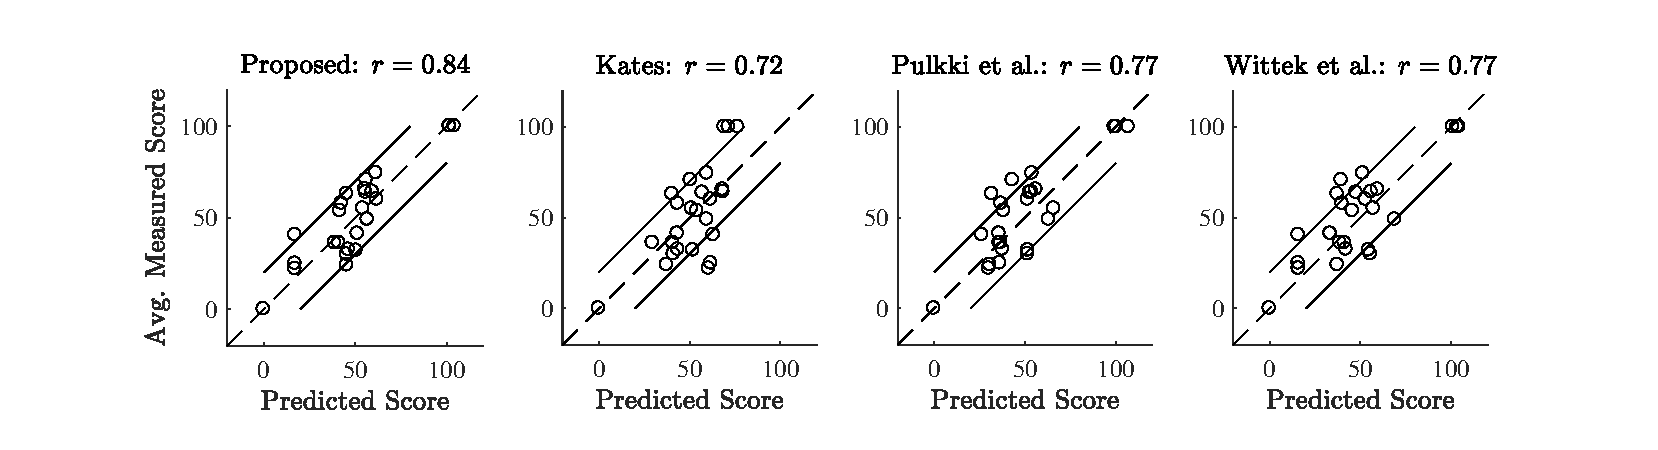
\includegraphics[width=0.99\textwidth,trim={2.15cm 0.3cm 2.3cm 0.5cm},clip]{05_proposed_models/figures/ColorationModelComparison}
  \caption[Scatter plots of average measured versus predicted coloration scores.]{
  Scatter plots of average measured versus predicted coloration scores for each model.
  The empty circles indicate the data and model values;
  the dashed lines indicate ideal model results (i.e., $y = x$);
  the solid lines indicate discrepancies of 20 points (i.e., $y = x \pm 20$).
  The predicted coloration scores for the binaural models (\citet{Pulkki1999} and \citet{Wittek2007}) are averaged across listeners.
  Correlation coefficients for each set of data are given at the top of each plot.}
  \label{fig:Coloration_Model_Comparison}
\end{figure}